\section{Results}
\label{sec:results}

This section reports the quantitative grid. Headline numbers are mean$\pm$std
across $10$ seeds (seeds $\{7, 11, 19, 23, 29, 31, 37, 41, 43, 47\}$, prime
numbers chosen at the start of the project). Sources are
\texttt{full\_mimic\_iv\_training/metrics/method\_summary.csv} for the original
run and \texttt{full\_mimic\_iv\_proposal\_alignment/metrics/proposal\_method\_summary.csv}
for the new run. We deliberately resist the temptation to declare a single
winner before Section~\ref{sec:mechanism}.

\subsection{Headline leaderboard, four metrics}
Table~\ref{tab:headline} is the four-metric leaderboard for the methods that
matter most. Bolded numbers are best in column.

\begin{table}[t]
\centering
\caption{Headline leaderboard. Mean$\pm$std over 10 seeds. Comm column in
millions of bytes (upload+download). All numbers from the CSVs cited above.}
\label{tab:headline}
\small
\begin{tabular}{lccccc}
\toprule
Method & Acc. & \auroc{} & \auprc{} & $\worstrec{}$ & Comm (Mb)\\
\midrule
\fedavg{} (default)        & $0.878\!\pm\!0.025$ & $0.889\!\pm\!0.008$ & $0.632\!\pm\!0.014$ & $0.21\!\pm\!0.14$ & $572$ \\
\cvar{}-$\alpha\!=\!0$      & $0.864\!\pm\!0.066$ & $0.886\!\pm\!0.013$ & $0.626\!\pm\!0.021$ & $\mathbf{0.26\!\pm\!0.21}^{\dagger}$ & $646$ \\
\cvar{}-$\alpha\!=\!0.5$    & $0.873\!\pm\!0.030$ & $0.876\!\pm\!0.014$ & $0.614\!\pm\!0.023$ & $0.16\!\pm\!0.13$ & $712$ \\
\cvar{}-$\alpha\!=\!0.75$   & $0.866\!\pm\!0.042$ & $0.878\!\pm\!0.019$ & $0.615\!\pm\!0.035$ & $0.24\!\pm\!0.14$ & $579$ \\
\cvar{}-$\alpha\!\geq\!0.9$$^*$ & $0.866\!\pm\!0.042$ & $0.878\!\pm\!0.019$ & $0.615\!\pm\!0.035$ & $0.24\!\pm\!0.14$ & $579$ \\
Centralized              & $\mathbf{0.908\!\pm\!0.004}$ & $0.878\!\pm\!0.007$ & $0.585\!\pm\!0.008$ & $0.16\!\pm\!0.13$ & $0$ \\
Local-only ($K=9$ models) & $0.904$ & $0.869$ & $0.459$ & $0.00$ & $0$ \\
Grid best                & $0.901\!\pm\!0.012$ & $0.859\!\pm\!0.030$ & $0.598\!\pm\!0.031$ & $0.13\!\pm\!0.13$ & $359$ \\
GA best                  & $0.867\!\pm\!0.051$ & $0.884\!\pm\!0.009$ & $0.629\!\pm\!0.012$ & $0.25\!\pm\!0.17$ & $\mathbf{318}$ \\
\midrule
\fedprox{}-$\mu\!=\!0$      & $0.889\!\pm\!0.016$ & $0.890\!\pm\!0.009$ & $0.636\!\pm\!0.010$ & $0.19\!\pm\!0.14$ & $442$ \\
\fedprox{}-$\mu\!=\!10^{-3}$ & $0.879\!\pm\!0.010$ & $0.902\!\pm\!0.005$ & $0.651\!\pm\!0.006$ & $0.41\!\pm\!0.18$ & $442$ \\
\fedprox{}-$\mu\!=\!10^{-2}$ & $0.861\!\pm\!0.010$ & $0.908\!\pm\!0.006$ & $0.660\!\pm\!0.012$ & $0.49\!\pm\!0.09$ & $592$ \\
\fedprox{}-$\mu\!=\!10^{-1}$ & $0.842\!\pm\!0.010$ & $\mathbf{0.913\!\pm\!0.001}$ & $\mathbf{0.665\!\pm\!0.005}$ & $\mathbf{0.50\!\pm\!0.05}$ & $428$ \\
\midrule
Logistic \fedavg{}        & $0.848\!\pm\!0.003$ & $0.895\!\pm\!0.001$ & $0.601\!\pm\!0.010$ & $0.45\!\pm\!0.07$ & $6.4$ \\
Logistic \fedprox{}-$\mu\!=\!0.1$ & $0.853\!\pm\!0.004$ & $0.899\!\pm\!0.002$ & $0.612\!\pm\!0.007$ & $0.45\!\pm\!0.07$ & $6.4$ \\
\bottomrule
\end{tabular}
\\[2pt]
\footnotesize
$^{\dagger}$ \cvar{}-$0$'s edge in worst-recall is fragile: std $0.21$ at mean $0.26$ implies $\sim40\%$ of seeds returned $0.0$.\quad
$^*$\cvar{}-$0.9$, $0.95$ are byte-identical to $0.75$ at $C\!=\!5$ -- see \S\ref{sec:mechanism-cvar}.
\end{table}

\begin{figure}[t]
    \centering
    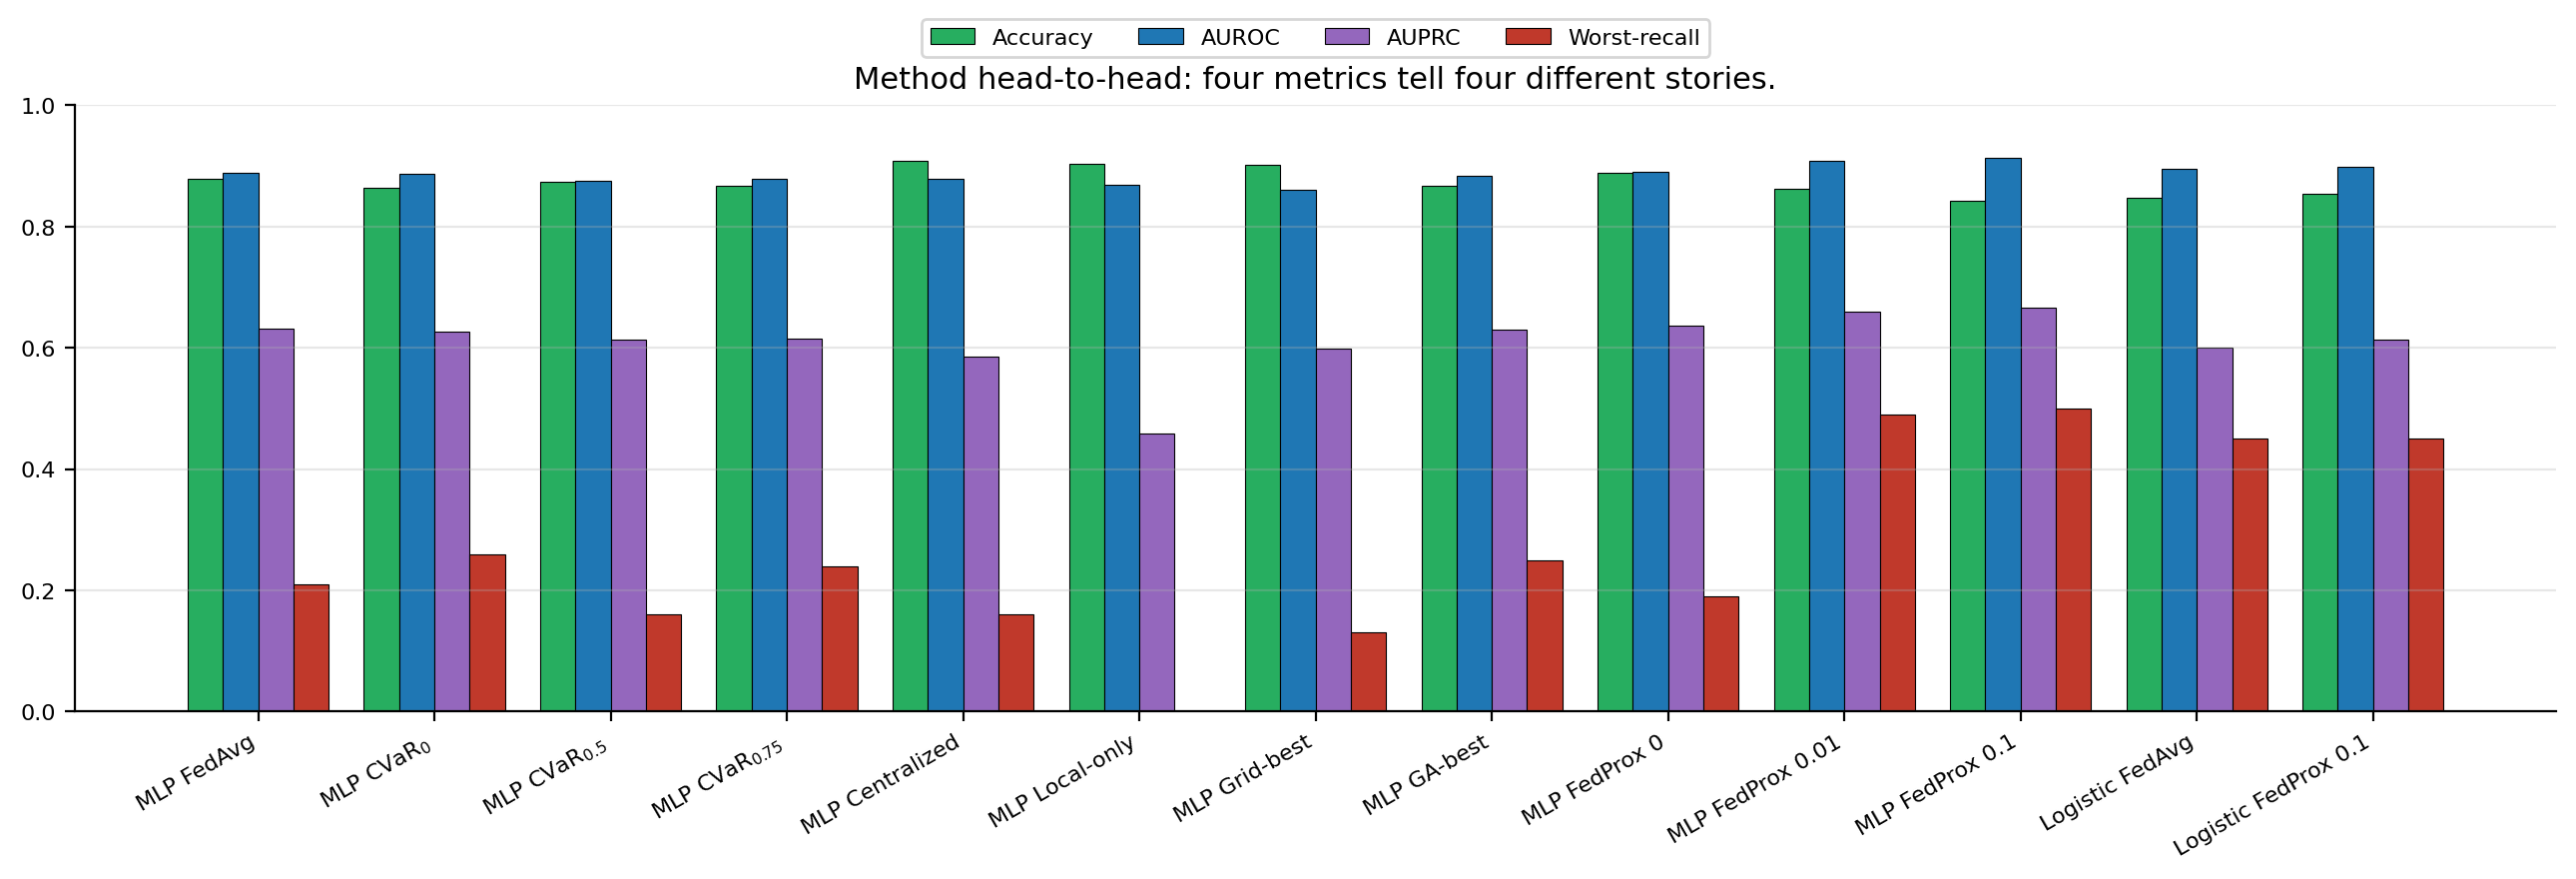
\includegraphics[width=\linewidth]{figures/fig_method_grouped_bars.png}
    \caption{Method head-to-head on four metrics. Centralized wins accuracy
        ($0.908$), \fedprox{}-$0.1$ wins \auroc{} ($0.913$) and \auprc{} ($0.665$),
        and \fedprox{}-$0.1$ also wins worst-client recall ($0.50$). The
        leaderboards \emph{disagree on what method is best}; the four metrics
        are not measuring the same thing.}
    \label{fig:headline-bars}
\end{figure}

\paragraph{Read this as four leaderboards, not one.}
\textbf{Accuracy:} Centralized wins ($0.908$), local-only is second ($0.904$),
grid-best third ($0.901$). Every federated method that explicitly fights
heterogeneity loses on accuracy because it gives up some MICU/MICU-SICU
correctness to recover the small Neuro units.

\textbf{\auroc{}:} \fedprox{}-$0.1$ wins ($0.913$). The four \fedprox{} variants
\emph{monotonically} climb the \auroc{} ladder with $\mu$, which is striking
because $\auroc{}$ is rank-based and supposedly insensitive to threshold.

\textbf{\auprc{}:} \fedprox{}-$0.1$ wins again ($0.665$), with the same monotone
shape. Centralized scores low ($0.585$) because it learns the average rate and
mis-ranks the rare class.

\textbf{Worst-client recall:} \fedprox{}-$0.1$ ties with \fedprox{}-$0.01$ at
$0.50 \pm 0.05$, double \fedavg{}'s $0.21$. \cvar{}-$0$ is nominally close but
its std reveals $\sim$40\% of seeds went to $0$, so it is not actually a
reliable fairness method.

\subsection{Per-seed reliability}
\begin{figure}[t]
    \centering
    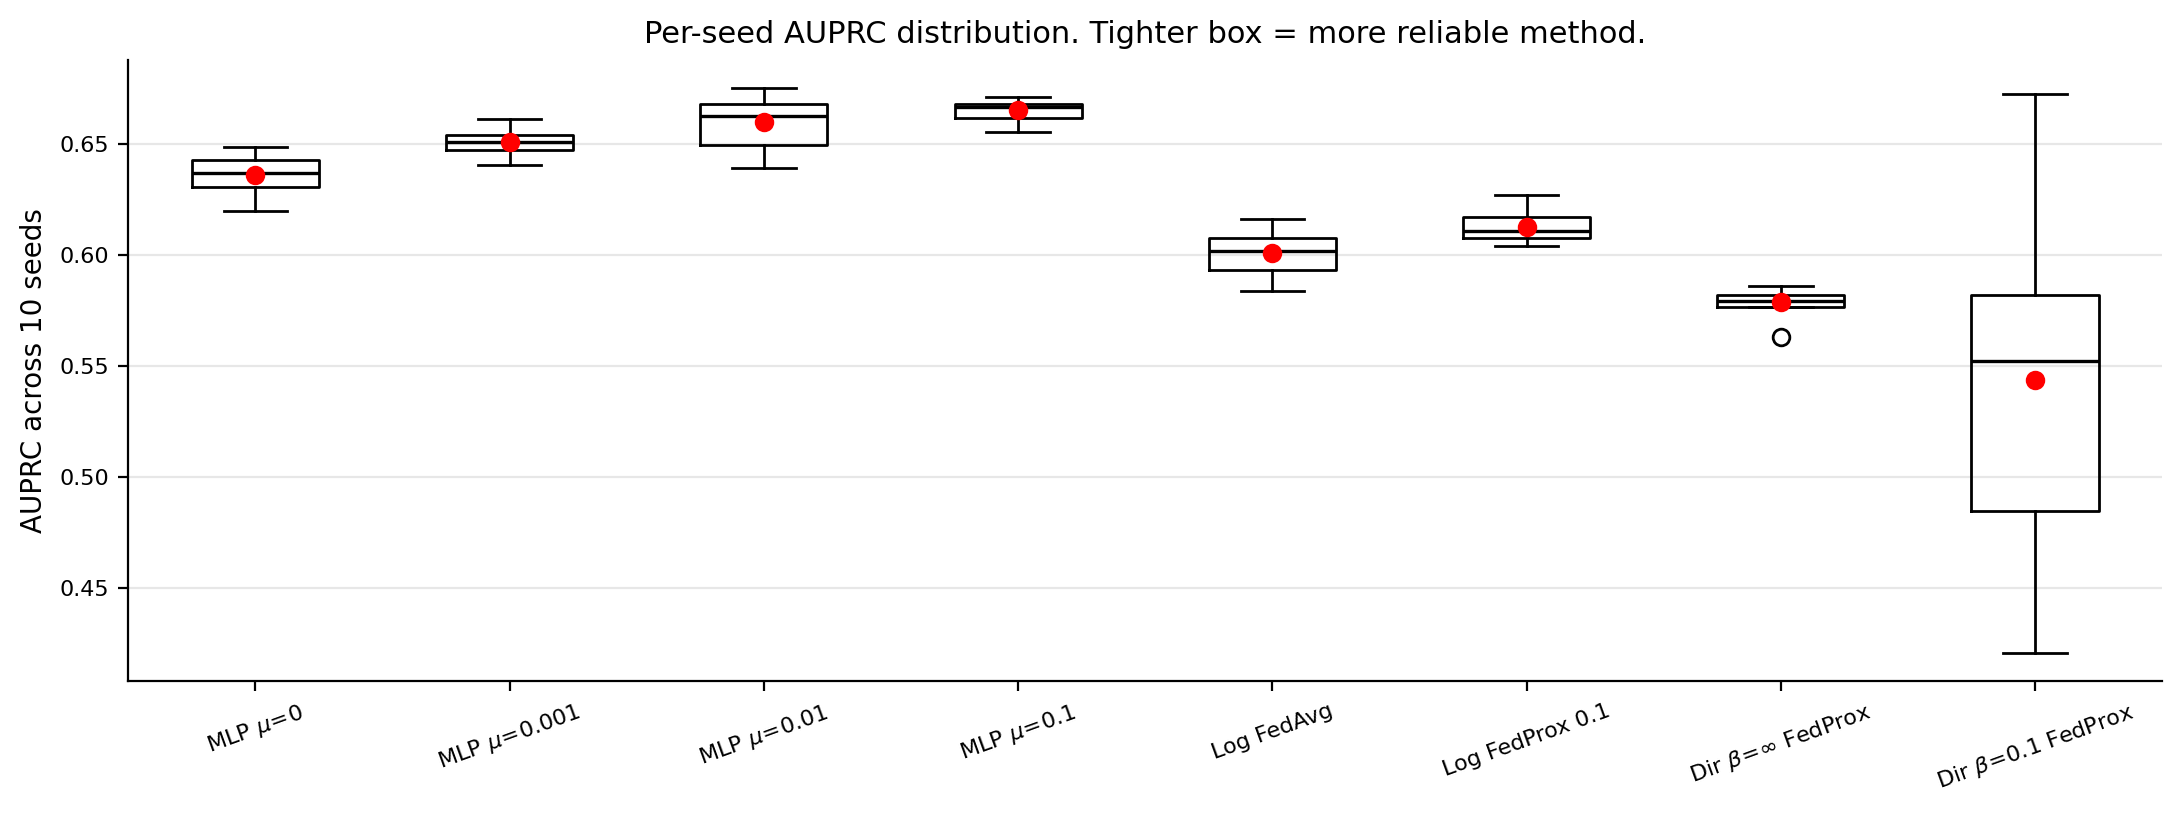
\includegraphics[width=\linewidth]{figures/fig_per_seed_auprc.png}
    \caption{Per-seed \auprc{} distributions for representative methods. The
        IQR width is the inverse reliability. \fedprox{}-$0.01$ and
        \fedprox{}-$0.1$ have the tightest boxes (std $\sim$$0.005$); the
        Dirichlet-$0.1$ box spans the entire vertical extent of the figure.}
    \label{fig:per-seed-auprc}
\end{figure}

The mean is not the whole story. Figure~\ref{fig:per-seed-auprc} shows that
\fedprox{}-$\mu\!\in\!\{0.01, 0.1\}$ achieve their gains \emph{reliably}: the
spread across seeds is so small that the IQR is barely visible. By contrast,
\fedavg{}'s box is taller (more across-seed variance), and the Dirichlet-$0.1$
box is enormous (across-seed std $0.113$, almost a quarter of the mean). This
tightening is part of what makes \fedprox{}-$0.1$ the deployment recommendation
even though its accuracy mean is lower.

\subsection{The Pareto frontier of \auprc{} vs.\ communication}
\begin{figure}[t]
    \centering
    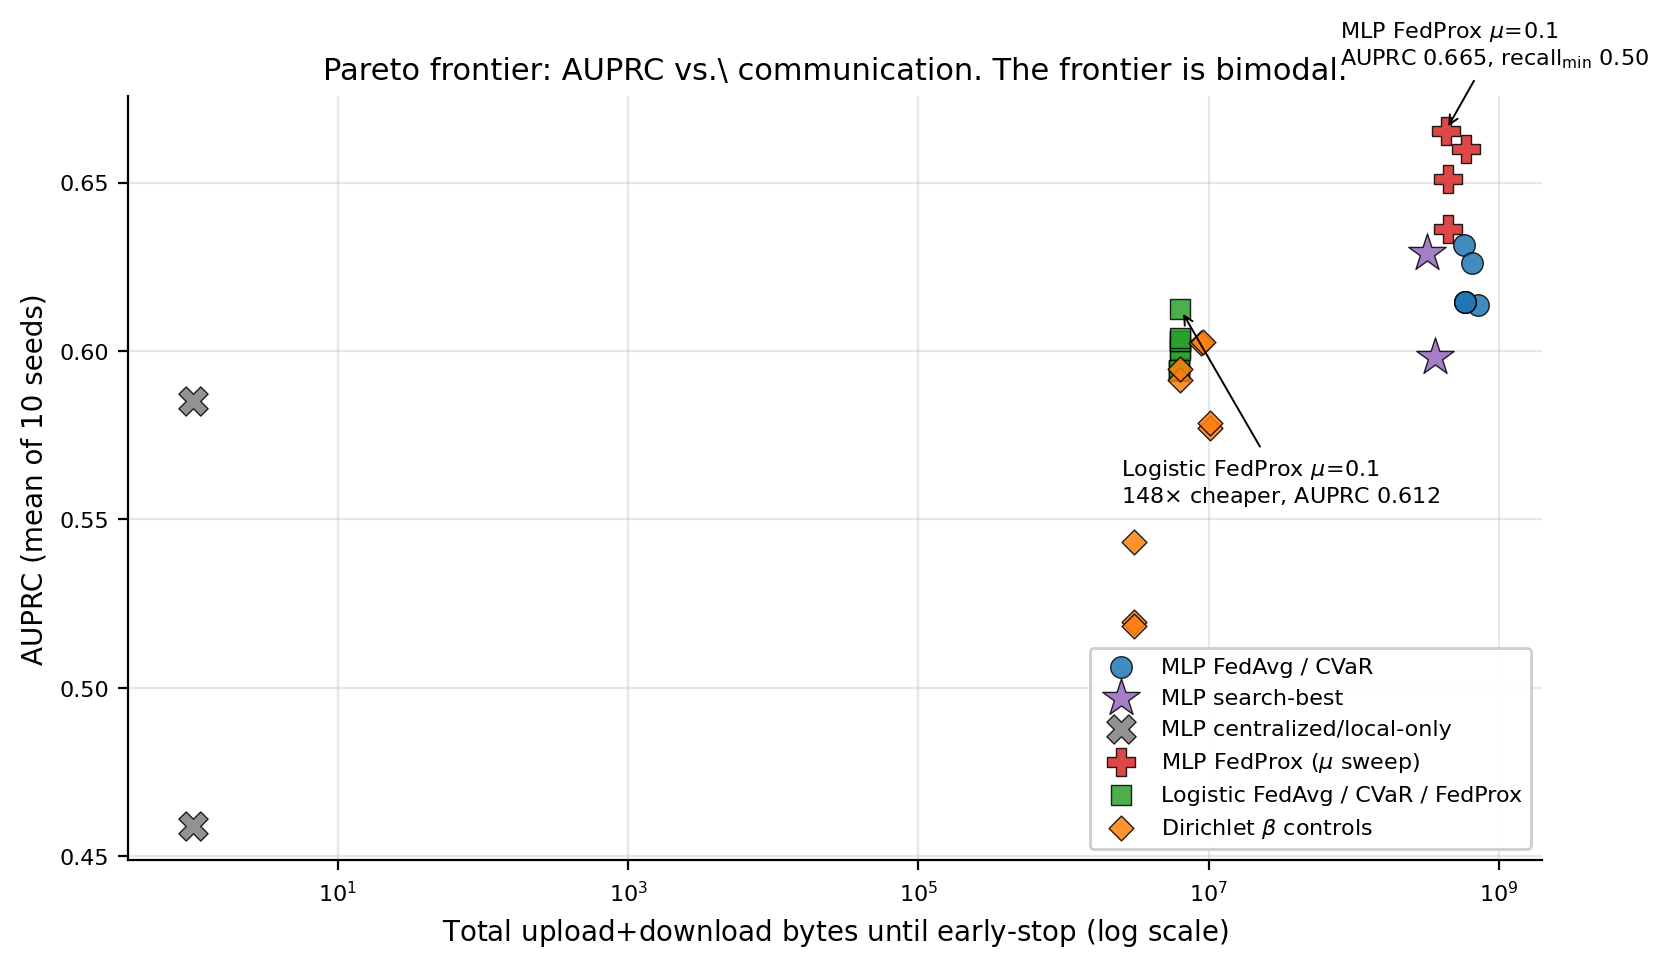
\includegraphics[width=\linewidth]{figures/fig_pareto_auprc_vs_comm.png}
    \caption{\auprc{}-vs-communication frontier. Two clusters: an MLP cluster
        at $\sim$$3$--$8\!\times\!10^8$ bytes and a logistic cluster at
        $6\!\times\!10^6$ bytes. The frontier between them is mostly empty
        (sparsity at $1\%$ would land in there). \fedprox{}-$0.1$ is the most
        north-east point on the MLP arc; logistic FedProx-$0.1$ is the
        most north-east point on the logistic arc.}
    \label{fig:pareto}
\end{figure}

The MLP cluster sits at $300$--$700$~MB; the logistic cluster at $6.4$~MB
($\sim$$50$--$110\!\times$ cheaper). The vertical gap between the two arcs is
$\auprc{}\!=\!0.665\,(MLP)$ vs.\ $0.612$ (logistic), \emph{i.e.}
$\Delta\auprc{}\!=\!0.053$ at $\sim 100\!\times$ communication. Whether that is
worth it is an operational decision; we discuss it in
Section~\ref{sec:clinical}. Top-$k$-compressed MLP (not run end-to-end but
projected by the LP) would land in the empty middle.

\subsection{Fairness frontier}
\begin{figure}[t]
    \centering
    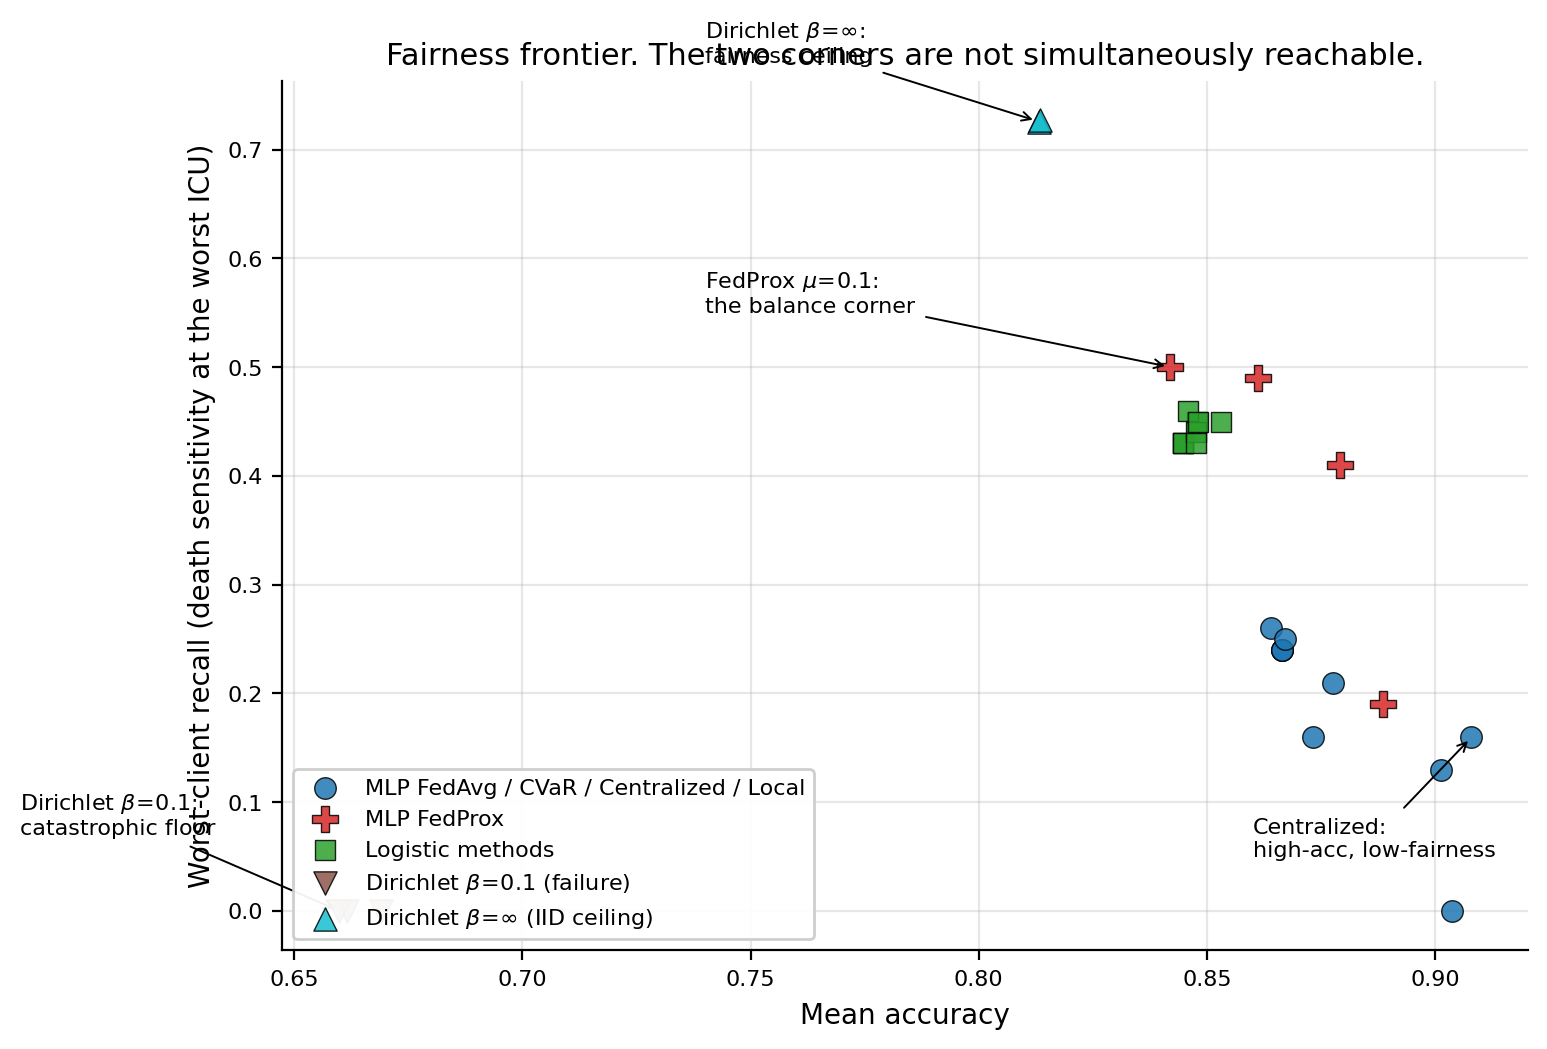
\includegraphics[width=0.85\linewidth]{figures/fig_fairness_frontier.png}
    \caption{Fairness frontier: mean accuracy vs.\ worst-client recall. The
        upper-right corner (high acc, high recall) is empty. The realised
        frontier is a clean L-shape: MLP-FedProx at $(0.84, 0.50)$, logistic
        FedAvg/FedProx at $(0.85, 0.45)$, and Centralized stuck at $(0.91,
        0.16)$. Dirichlet-$0.1$ is below everything; Dirichlet-$\infty$
        provides the IID ceiling.}
    \label{fig:fairness-frontier}
\end{figure}

The empty upper-right corner of Figure~\ref{fig:fairness-frontier} is the
single most important visual in the report. \emph{No method we tried gets both
high mean accuracy and high worst-client recall on natural clients}, including
the centralized baseline. The reason is structural -- it is the same
heterogeneity that drives every other result -- and the only knob that breaks
the trade-off is reducing heterogeneity itself (Dirichlet-$\infty$).

\subsection{Heterogeneity sweep (Dirichlet)}
\begin{figure}[t]
    \centering
    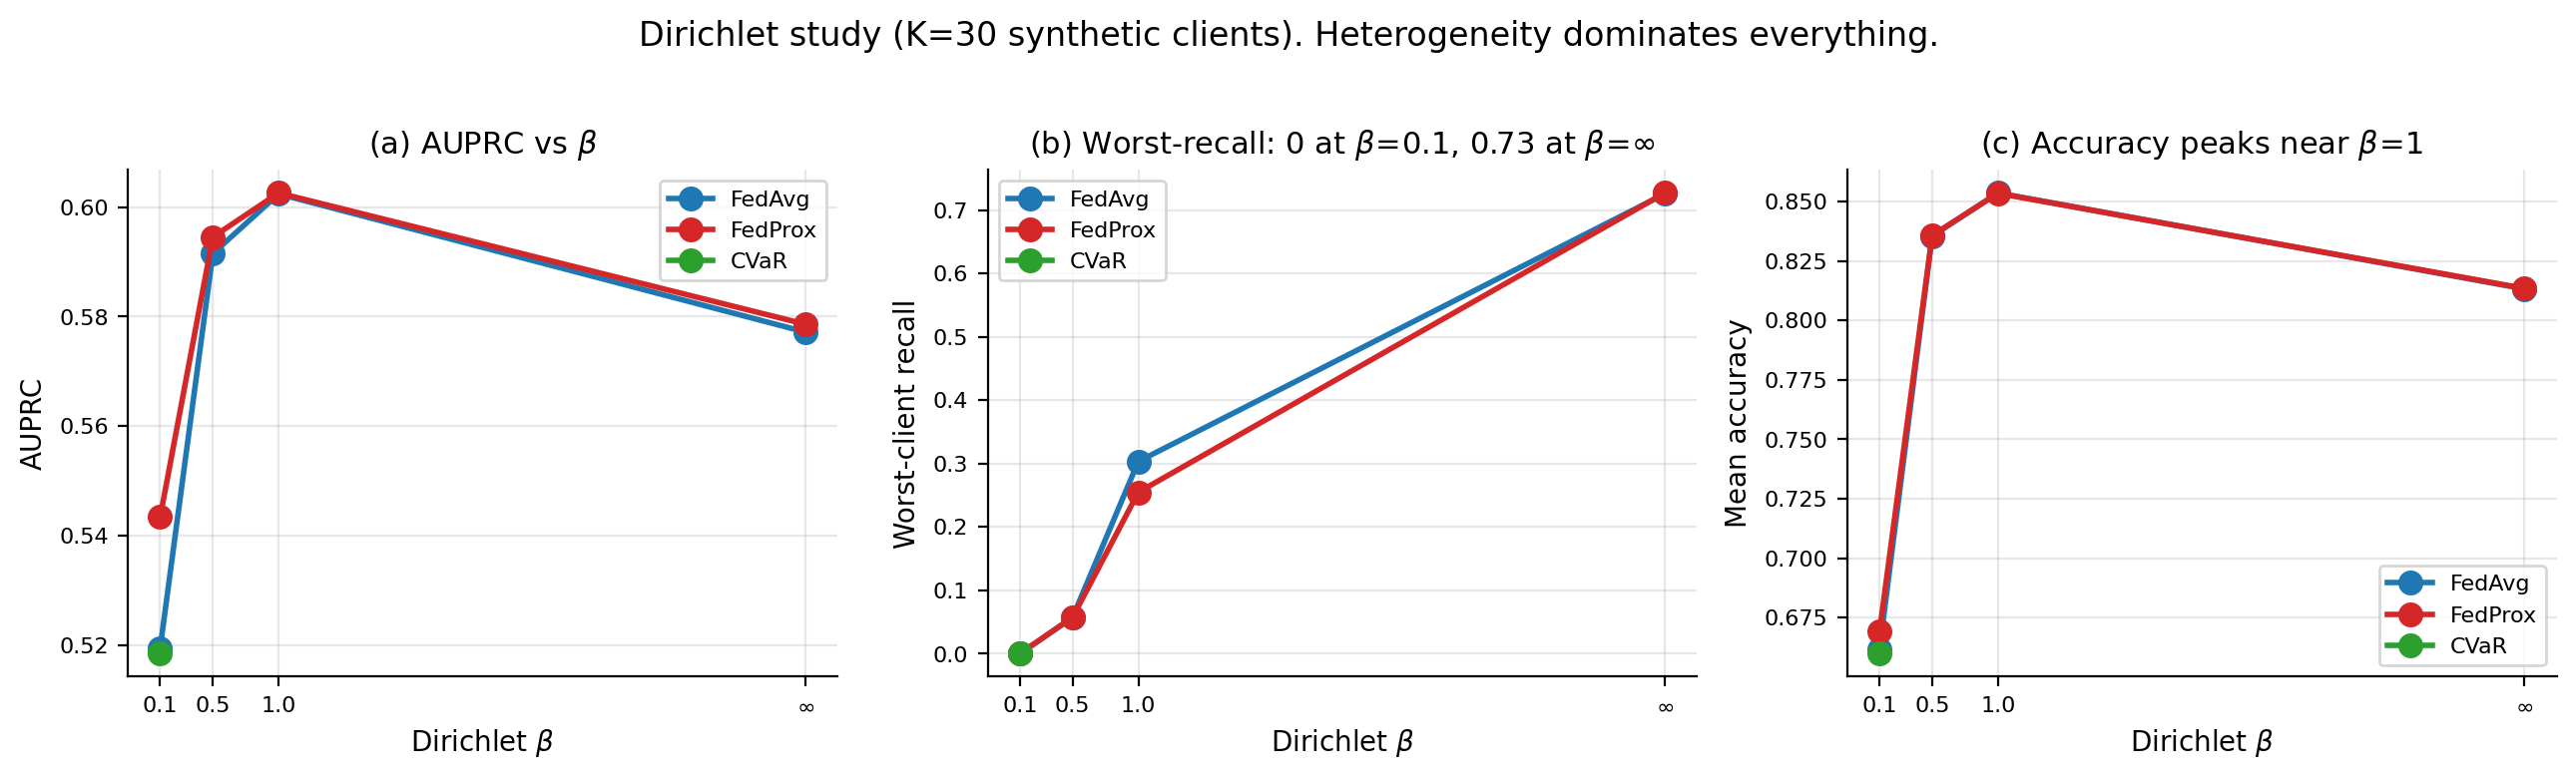
\includegraphics[width=\linewidth]{figures/fig_dirichlet_trends.png}
    \caption{Dirichlet $\beta$ sweep, $K\!=\!30$ synthetic clients.
        $\beta \!=\! 0.1$ is catastrophic for every method;
        $\beta \!=\! \infty$ (IID) is the ceiling for every method.
        FedAvg and FedProx are statistically indistinguishable here -- the
        \emph{heterogeneity axis dominates the algorithm axis}. CVaR
        underperforms FedAvg on \auprc{} when heterogeneity is high.}
    \label{fig:dirichlet}
\end{figure}

Three observations:
\begin{enumerate}[leftmargin=*,nosep]
    \item At $\beta \!=\! 0.1$ all three algorithms collapse to
        $\auprc{} \in [0.52, 0.55]$ and worst-recall $0$. This is the
        federated failure regime; no algorithm rescues it.
    \item At $\beta \!=\! \infty$ all three algorithms recover to worst-recall
        $\sim 0.73$, the highest worst-recall observed in the entire study.
        The IID regime makes the per-client minima coincide; the federated
        objective becomes the centralized objective and the rare class is no
        longer geographically concentrated.
    \item FedProx and FedAvg trace each other almost exactly across $\beta$,
        within their own seed-std. This confirms that the proximal term's
        \emph{role} is dampening drift, and at $\beta \!=\! \infty$ there is no
        drift to dampen.
\end{enumerate}

\subsection{Hyperparameter search}
\begin{figure}[t]
    \centering
    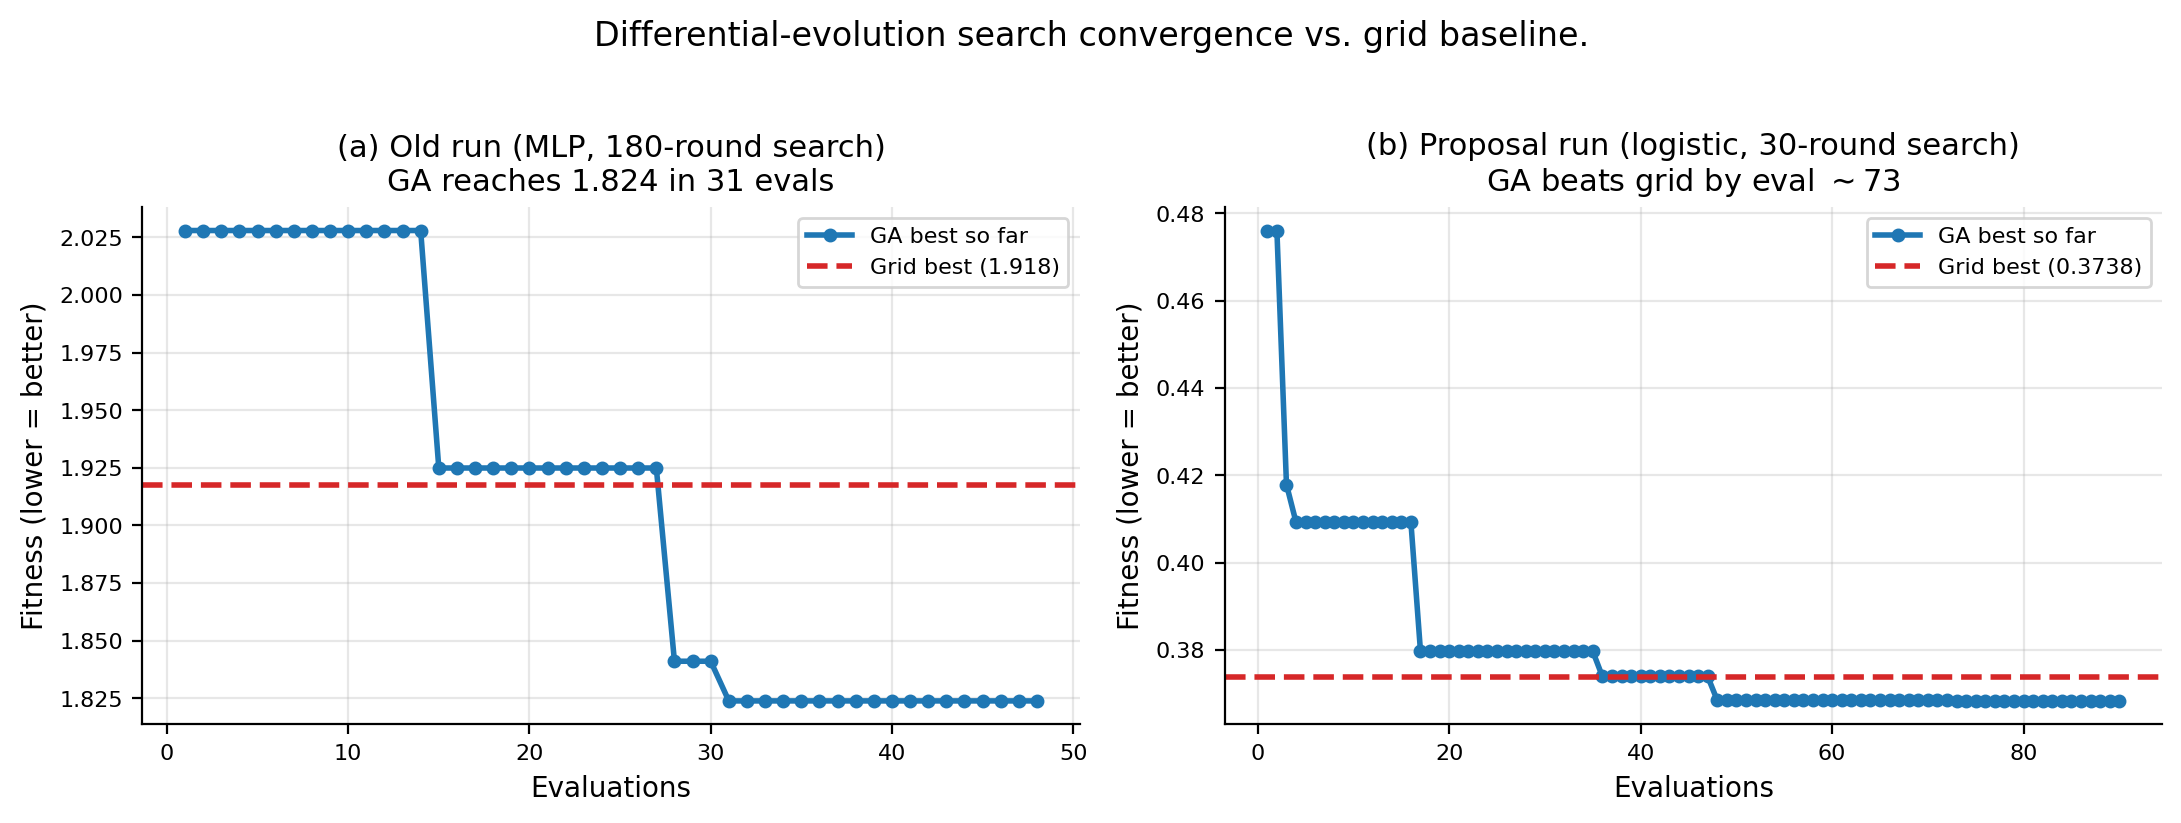
\includegraphics[width=\linewidth]{figures/fig_ga_convergence.png}
    \caption{DE search vs.\ grid baseline. Left (old MLP run): GA converges to
        fitness $1.824$ in $31$ evaluations; grid best is $1.918$. Right
        (proposal logistic run): GA converges to $0.368$ in $73$ evaluations;
        grid best is $0.374$. Both runs show GA finding an off-grid optimum
        that grid by construction cannot.}
    \label{fig:ga-convergence}
\end{figure}

GA wins on both runs. The proposal-run winning configuration is
$E\!=\!2.52, C\!=\!3.74, \eta\!=\!0.0029$
(\texttt{search/proposal\_ga\_result.json:x}). The off-grid $\eta\!=\!0.0029$
is the precise reason: the grid had only $\{0.003, 0.005, 0.01\}$ available.
We expand on this in \S\ref{sec:mechanism-search}.

\begin{figure}[t]
    \centering
    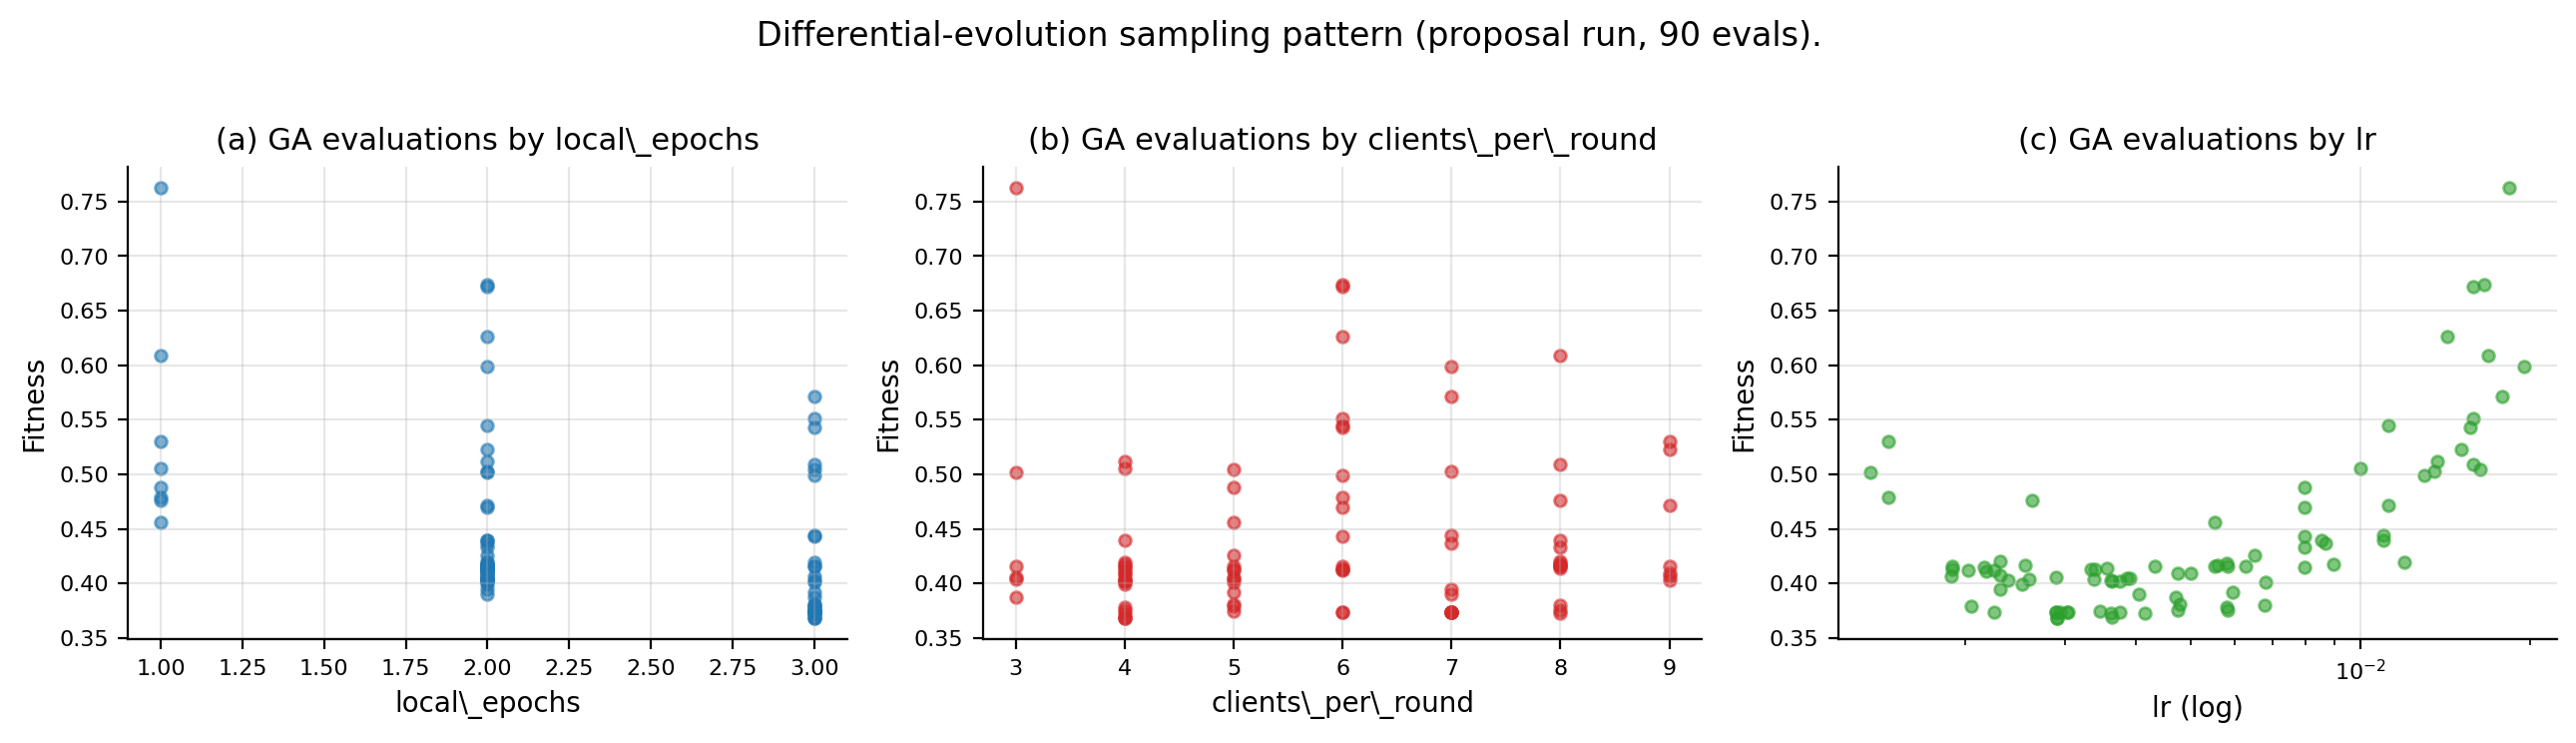
\includegraphics[width=\linewidth]{figures/fig_search_history_scatter.png}
    \caption{Per-axis fitness scatter for the proposal-run DE history.
        Fitness has the cleanest dependence on $\eta$: log-$\eta < 10^{-2.5}$
        gives the lowest fitnesses. $E$ and $C$ are nearly orthogonal to
        fitness in this range -- the model is not bottlenecked by either.}
    \label{fig:ga-scatter}
\end{figure}

\subsection{LP duality and sparsity}
\begin{figure}[t]
    \centering
    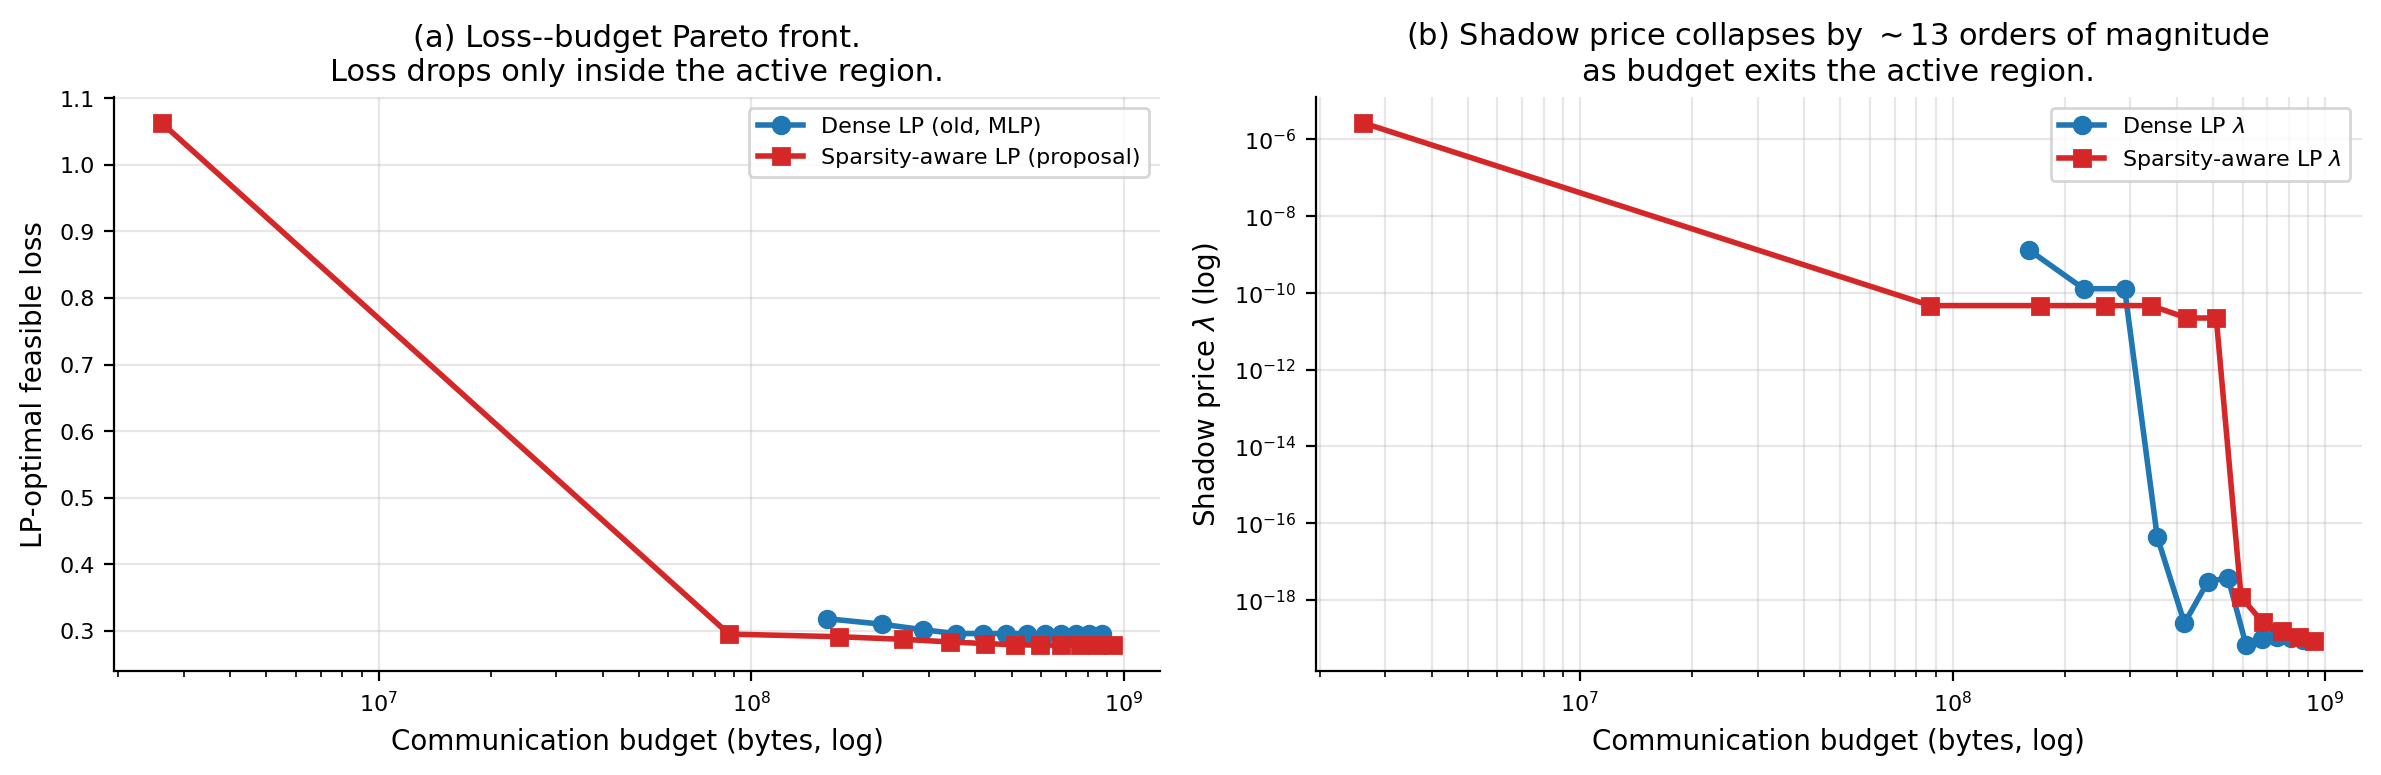
\includegraphics[width=\linewidth]{figures/fig_lp_shadow_price.png}
    \caption{LP shadow-price program. Left: loss vs.\ budget. Both dense and
        sparse formulations carve a clean Pareto frontier in the active region
        and saturate. Right: shadow price $\lambda$. The $13$-order-of-magnitude
        cliff between active and saturated regions is the LP saying ``one
        configuration is bytes-optimal; further budget pays for itself only
        marginally.''}
    \label{fig:lp-shadow}
\end{figure}

\begin{figure}[t]
    \centering
    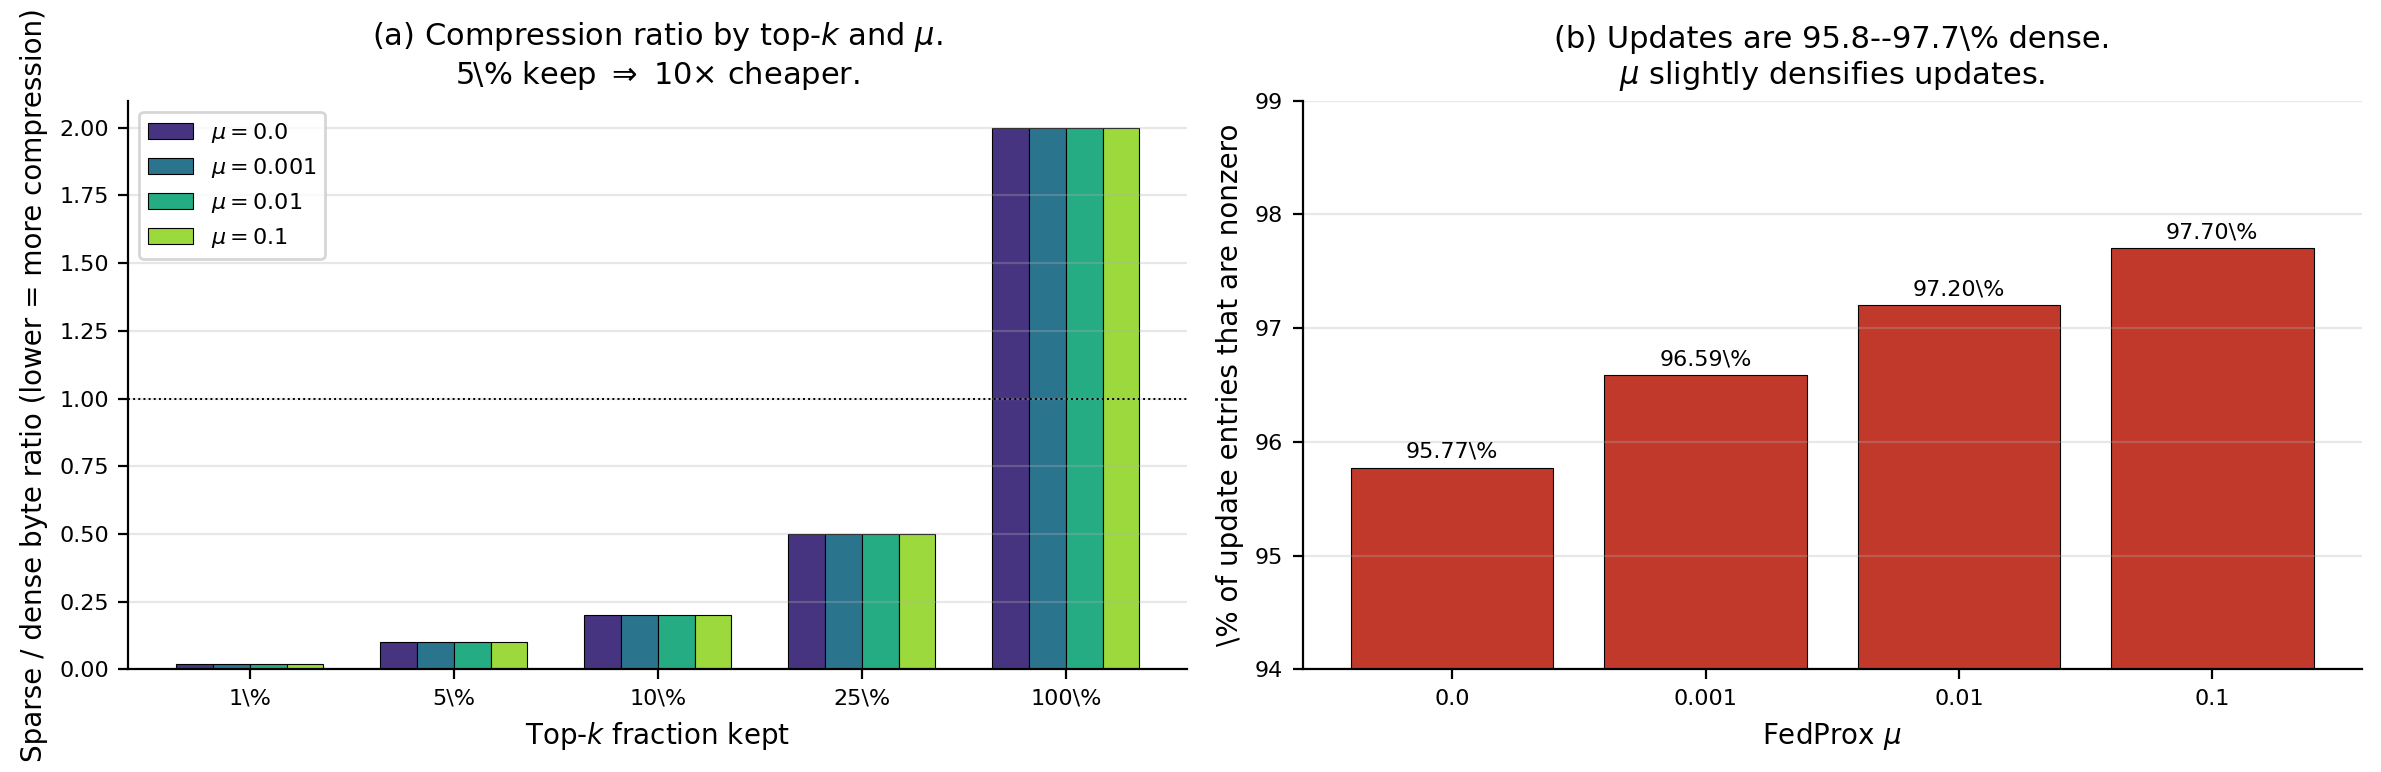
\includegraphics[width=\linewidth]{figures/fig_sparsity_compression.png}
    \caption{Top-$k$ compression diagnostics. Left: byte-ratio for $k\!\in\!\{1,5,10,25,100\}\%$
        and $\mu\!\in\!\{0,0.001,0.01,0.1\}$, ratios are essentially insensitive
        to $\mu$. Right: natural sparsity. Updates are $95.8$--$97.7\%$
        nonzero, increasing slightly with $\mu$. Compression is therefore
        \emph{lossy truncation}, not free natural sparsity.}
    \label{fig:sparsity}
\end{figure}

The LP says: spend bytes only inside the active region. The sparsity
diagnostic says: top-$k$ at $5\%$ is roughly $10\!\times$ cheaper, but this
costs accuracy because there is no natural sparsity to exploit -- the model
\emph{wants} those entries. We do not run end-to-end top-$k$ training (it would
require a separate run; left to future work, \S\ref{sec:future}).

\subsection{Loss landscape}
\begin{figure}[t]
    \centering
    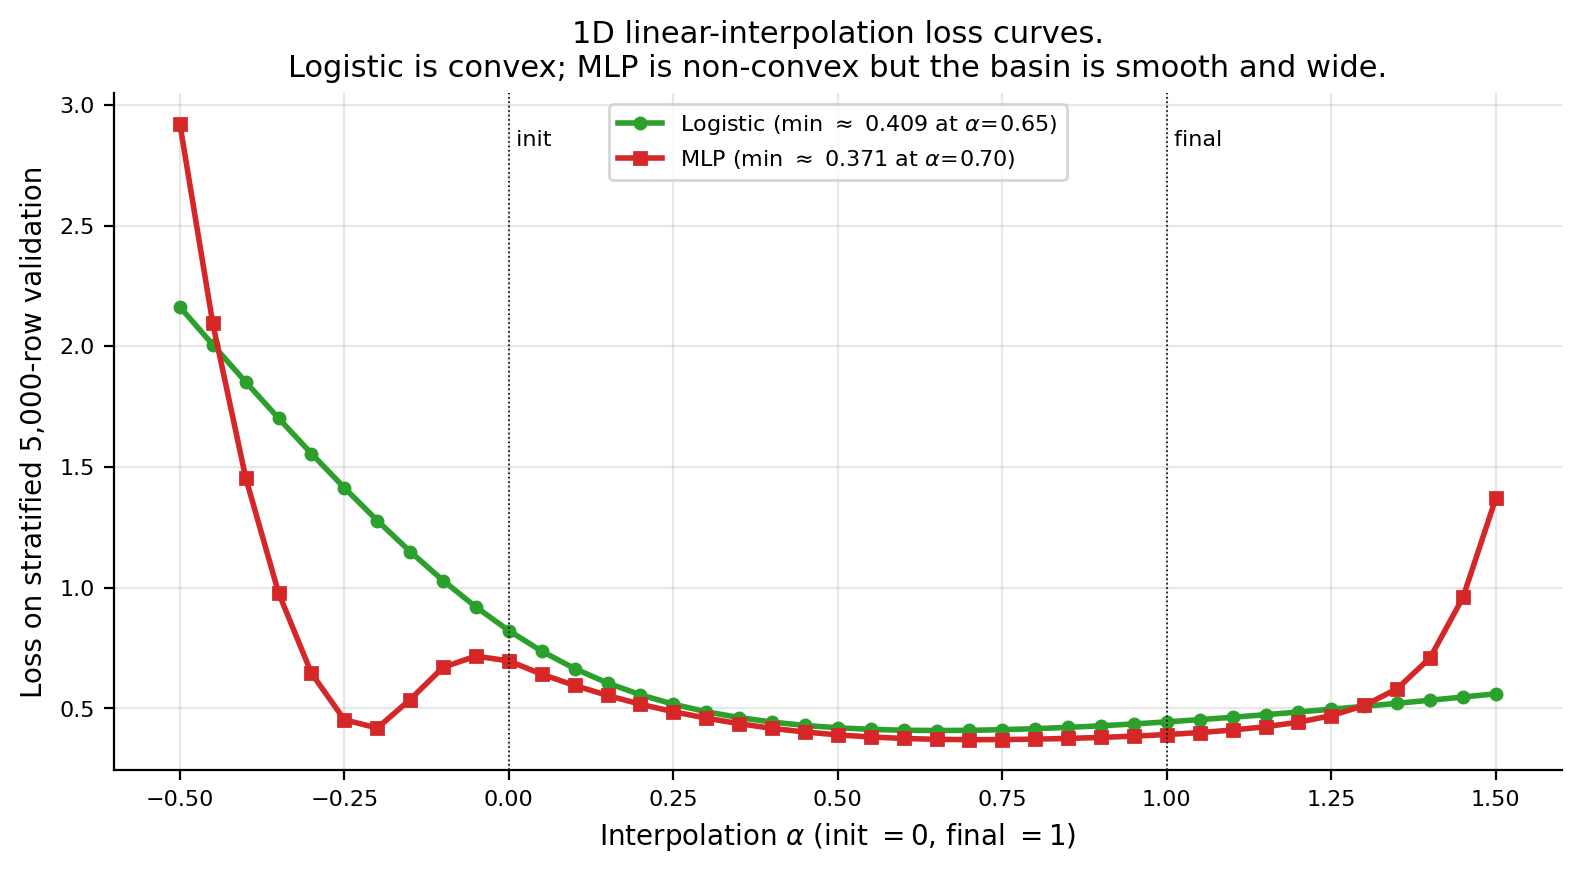
\includegraphics[width=\linewidth]{figures/fig_loss_landscape_1d.png}
    \caption{1D linear-interpolation curves. Logistic has the textbook convex
        U-shape; min at $\alpha\!=\!0.65, \mathrm{loss}\!=\!0.409$. MLP is
        non-convex but the basin from $\alpha\!\sim\!0.05$ to $\alpha\!\sim\!1.2$
        is smooth and wide (loss $\in [0.371, 0.49]$). The bump near
        $\alpha\!\in\![-0.10, 0]$ is small but real; we discuss it in
        \S\ref{sec:mechanism-landscape}.}
    \label{fig:landscape-1d}
\end{figure}

\begin{figure}[t]
    \centering
    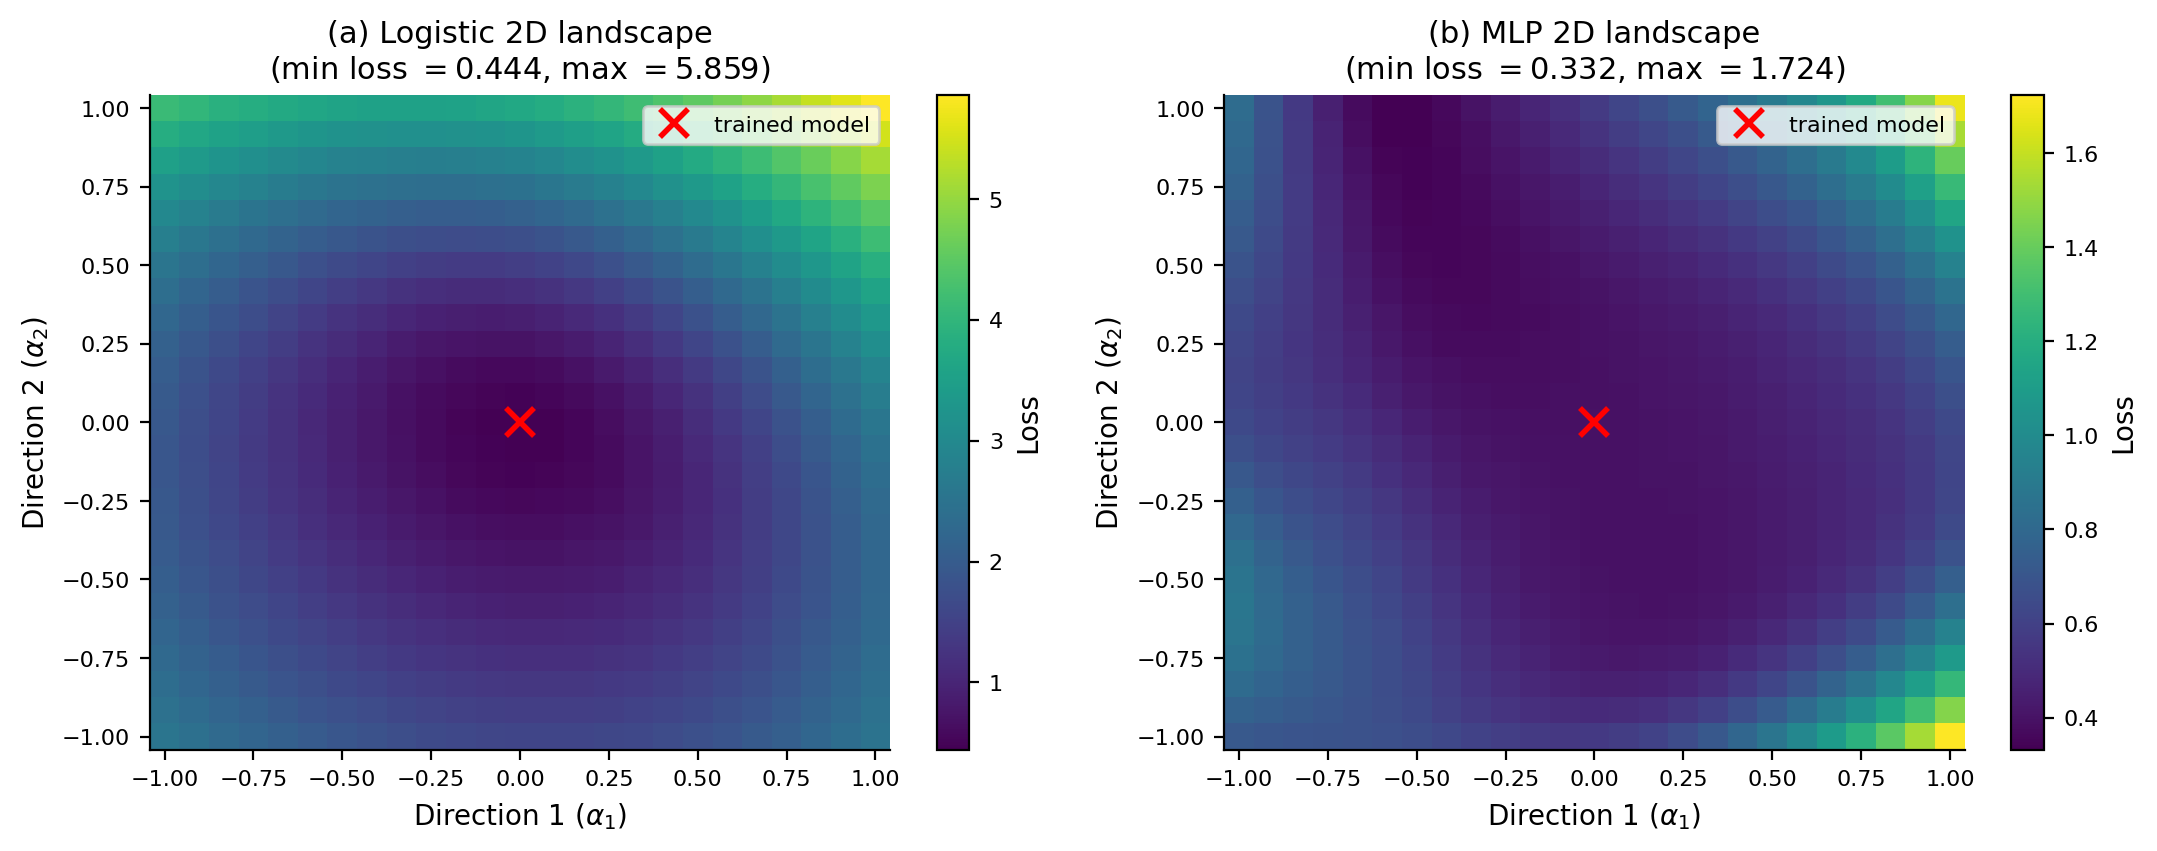
\includegraphics[width=\linewidth]{figures/fig_loss_landscape_2d.png}
    \caption{2D filter-normalized landscapes. Logistic (a) is a clean basin.
        MLP (b) is also a clean basin near the trained model
        ($\alpha_1\!=\!\alpha_2\!=\!0$); steep boundaries appear at the corners
        because the model is many standard deviations away from any local min.
        Min loss in the rendered window: logistic $0.41$, MLP $0.37$.}
    \label{fig:landscape-2d}
\end{figure}

\subsection{Best validated MLP: clinical breakdown}
The best validated configuration (the row written to
\texttt{method\_summary.csv:grid\_best\_validated}) achieves the test-set
metrics in Table~\ref{tab:clinical-best}.

\begin{table}[t]
\centering
\caption{Test-set metrics for the best validated MLP.}
\label{tab:clinical-best}
\small
\begin{tabular}{lc lc}
\toprule
Accuracy & $0.840$ & Sensitivity & $0.784$\\
Balanced acc.\ & $0.816$ & Specificity & $0.848$\\
\auroc{} & $0.905$ & Precision (PPV) & $0.398$\\
\auprc{} & $0.653$ & NPV & $0.968$\\
F1 (death) & $0.528$ & Brier & $0.113$\\
Mean confidence & $0.821$ & ECE & $0.019$\\
\bottomrule
\end{tabular}
\end{table}

\begin{figure}[t]
    \centering
    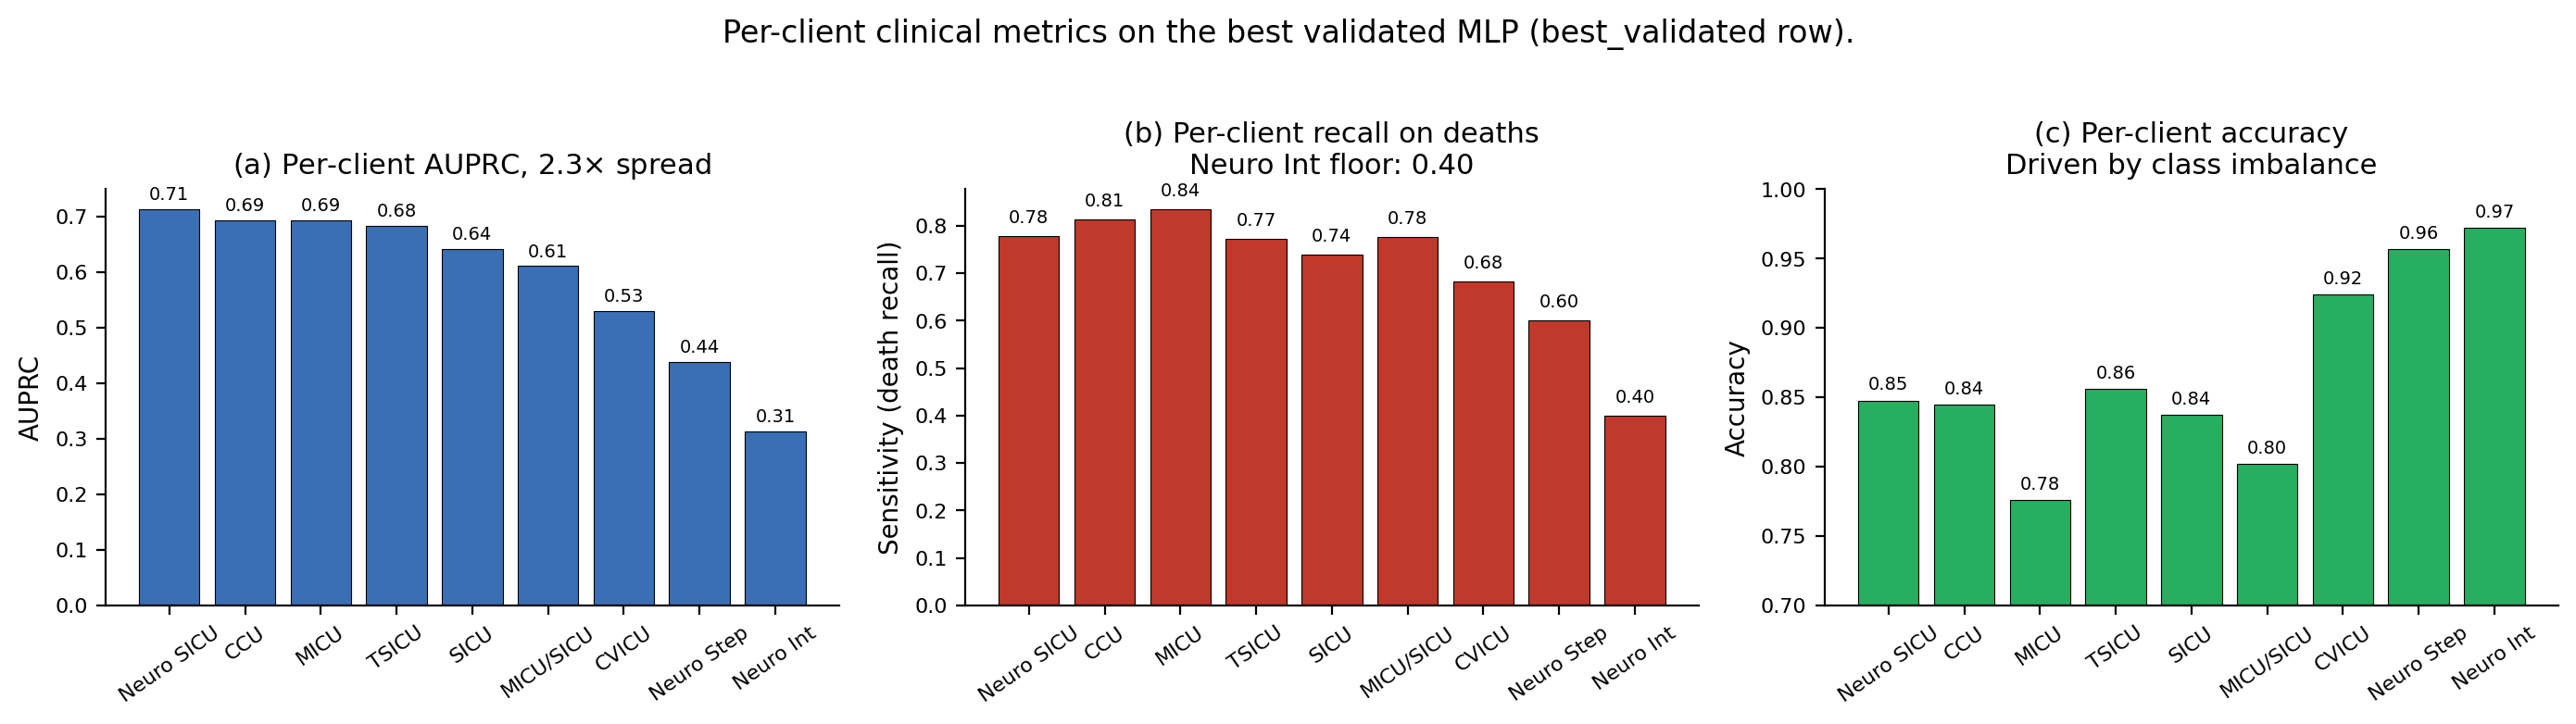
\includegraphics[width=\linewidth]{figures/fig_per_client_clinical.png}
    \caption{Per-client clinical metrics on the best validated MLP. Best
        AUPRC: Neuro SICU $0.71$. Worst: Neuro Intermediate $0.31$. The 2.3$\!\times$
        spread is purely a function of how many positives each ICU has (Neuro
        Int has 10 deaths in the test fold; Neuro SICU has 72).}
    \label{fig:per-client-clinical}
\end{figure}

\begin{figure}[t]
    \centering
    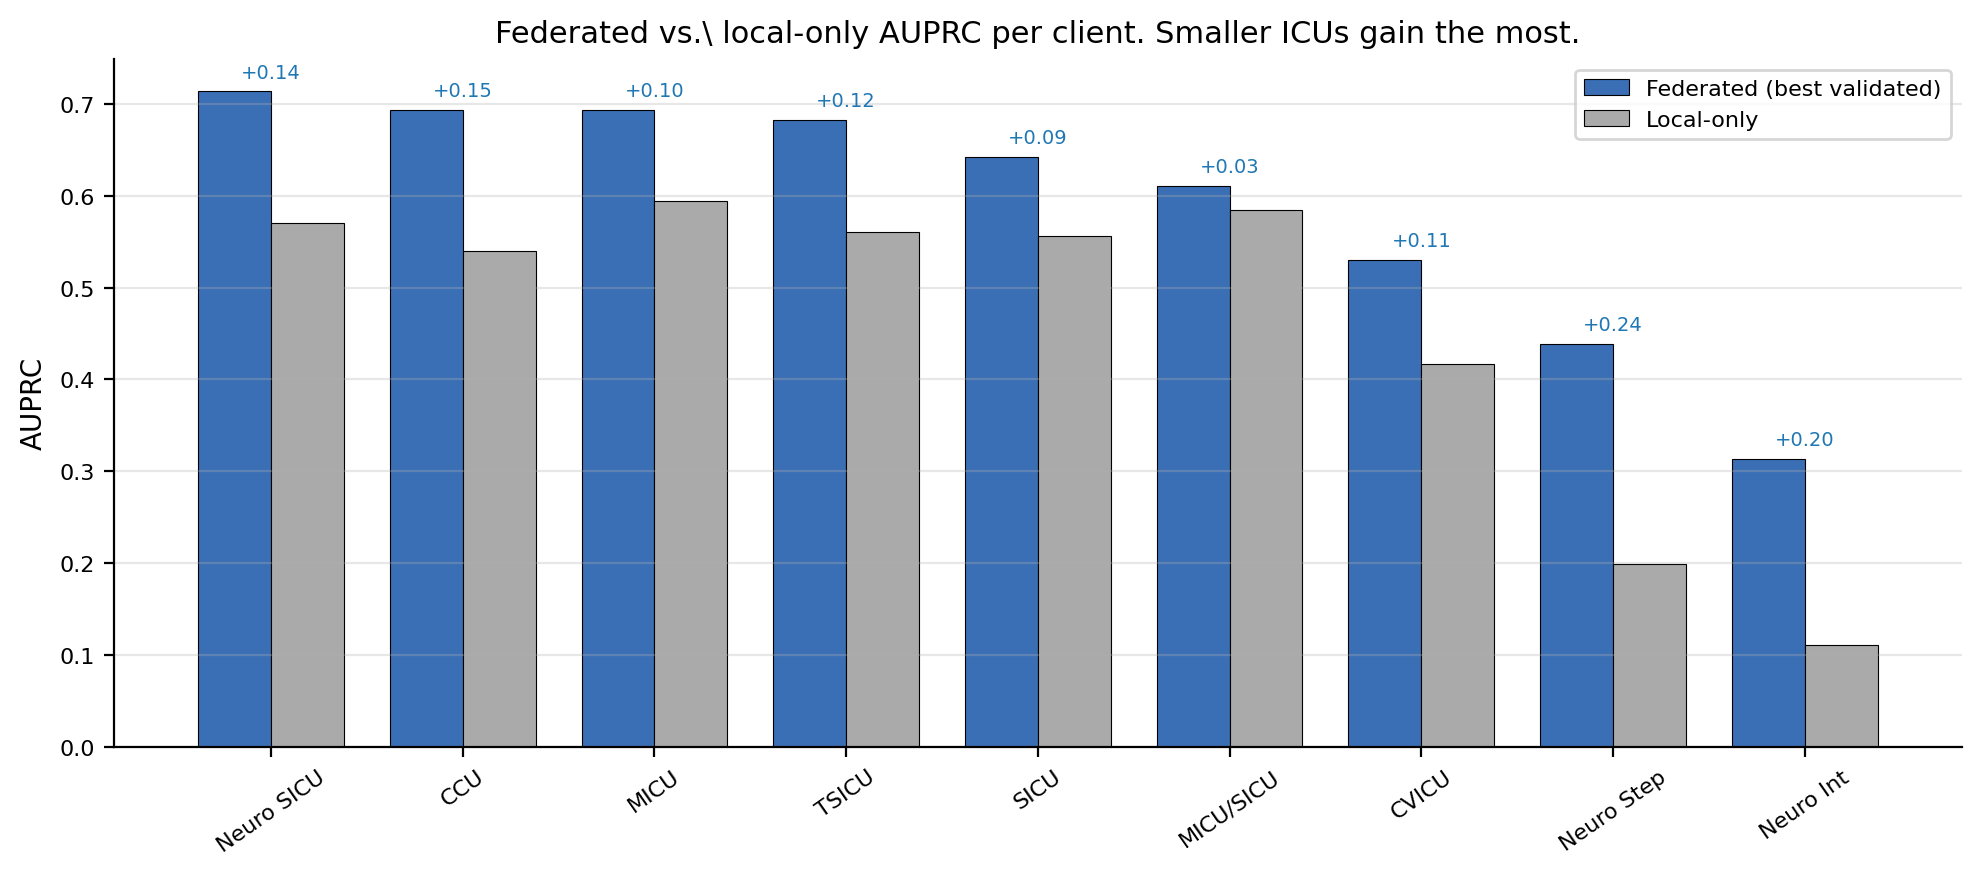
\includegraphics[width=\linewidth]{figures/fig_local_vs_fed_per_client.png}
    \caption{Federation gain over local-only, per client. Every client gains
        \auprc{}; the smallest units gain the most ($+0.32$ at Neuro Stepdown,
        $+0.21$ at Neuro Intermediate). MICU is the smallest gainer ($+0.07$)
        because its local data is already plentiful. \emph{The federation pays
        off for the smallest clients, exactly as predicted by the heterogeneity
        analysis.}}
    \label{fig:local-vs-fed}
\end{figure}

\begin{figure}[t]
    \centering
    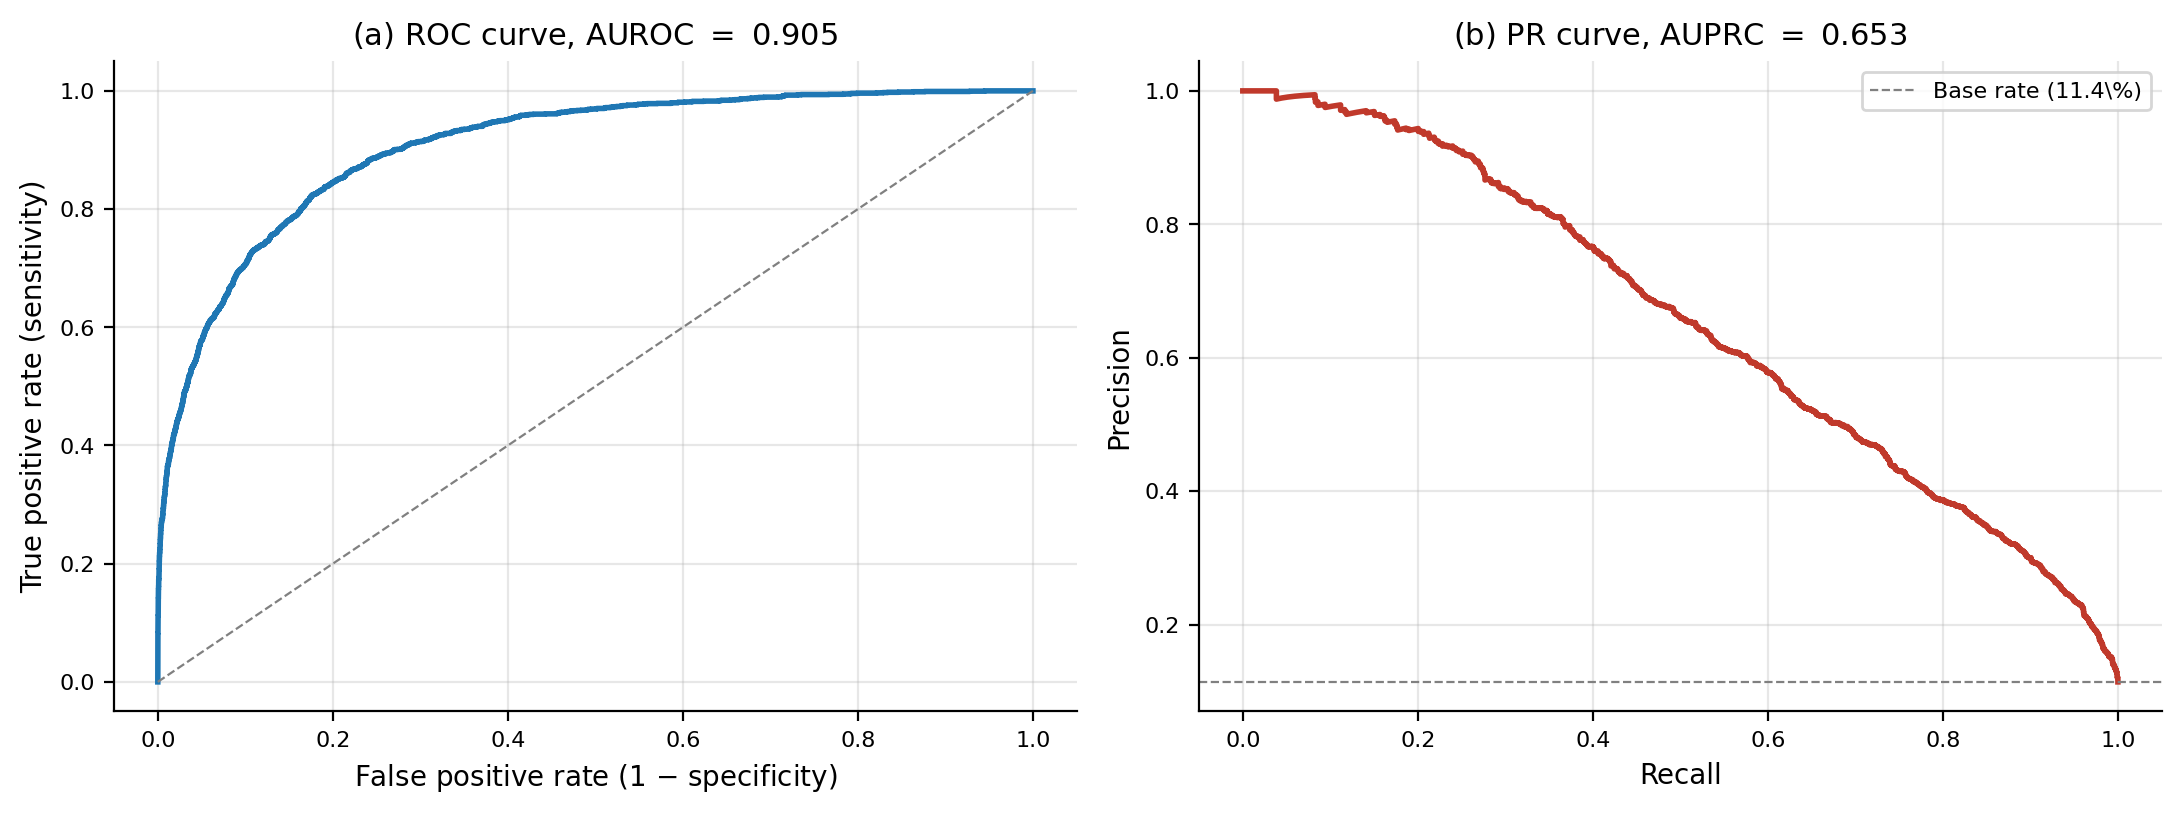
\includegraphics[width=\linewidth]{figures/fig_roc_pr_curves.png}
    \caption{ROC and PR curves on the best validated MLP. AUROC $=0.905$,
        AUPRC $=0.653$. The PR curve sits well above the $11.4\%$ base
        rate.}
    \label{fig:roc-pr}
\end{figure}

\begin{figure}[t]
    \centering
    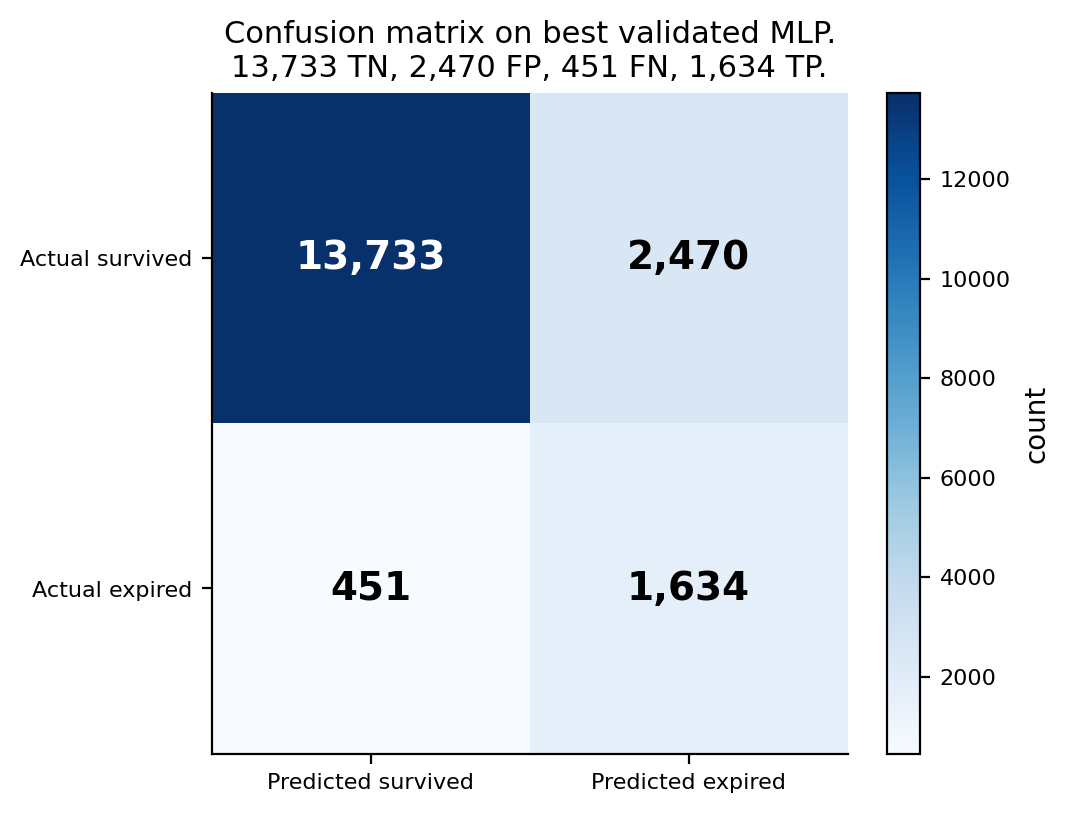
\includegraphics[width=0.65\linewidth]{figures/fig_confusion_matrix.png}
    \caption{Confusion matrix on the best validated MLP. The $451$ false
        negatives are the most clinically expensive number in this report:
        $451$ patients who died but were classified as ``survived.'' The model
        catches $1{,}634$ of $2{,}085$ deaths ($78.4\%$).}
    \label{fig:cm}
\end{figure}

\subsection{Operational footprint}
\begin{figure}[t]
    \centering
    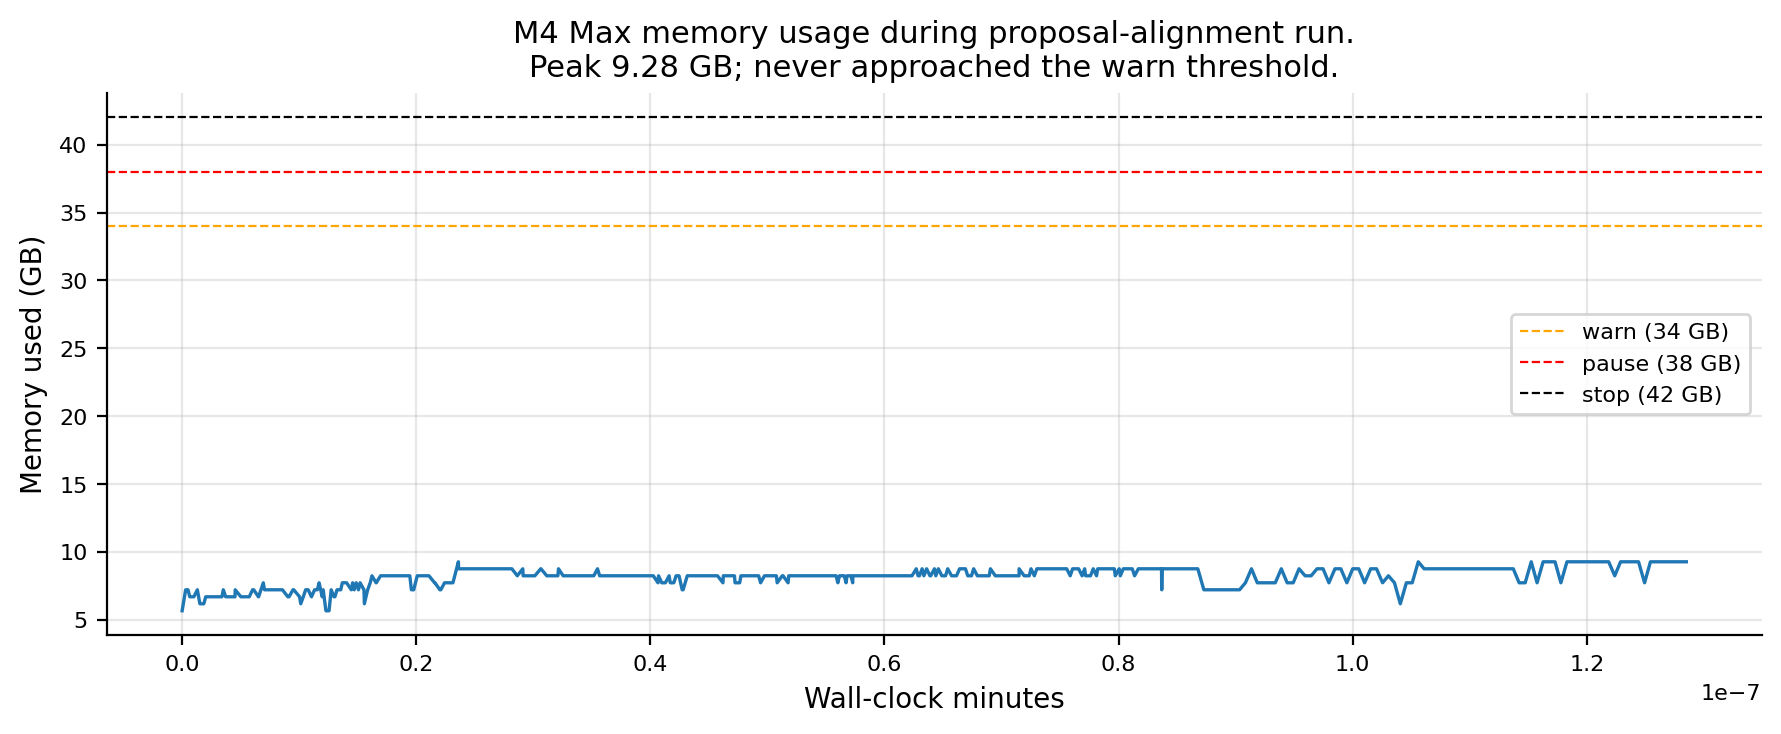
\includegraphics[width=0.85\linewidth]{figures/fig_resource_timeseries.png}
    \caption{Memory usage during the proposal-alignment run on M4 Max 48~GB.
        Peak usage $9.3$~GB; the warn/pause/stop guardrails at $34/38/42$~GB
        were never triggered. The watchdog logged $477$ samples without
        intervention.}
    \label{fig:resources}
\end{figure}

The full run completed without OOM, swap thrash, or watchdog intervention. The
peak memory of $9.3$~GB is dominated by feature matrices in DuckDB cache and
PyTorch tensors; the model itself is sub-megabyte
(\texttt{outputs/full\_mimic\_iv\_proposal\_alignment/monitoring/resource\_summary.csv}).
